%% thesis.tex
%% Distributed with umalayathesis v1.5.1 (1 June 2020)
\documentclass[english,singlespacedlisttitles]{umalayathesis}
%% Document class options
%% -----------------------
%% english (default): English thesis
%%
%% bahasam : Malay thesis
%%
%% apacite (default): Loads the apacite package, which implements the APA
%%    citation and referencing styles strictly. Now caters for APA7 so will
%%    not expand full author list for items with 3–5 authors (rejoice!)
%%
%% custombib: Does not pre-load any bibliography style; you will need to
%%    specify \bibliographystyle, \bibliographystyleown etc yourself.
%%
%% appendixhead: Add "APPENDICES" before the Appendix A title
%%
%% altcaption: Caption in smaller fonts; only Figure X, Table Y bold.
%%
%% singlespacedlisttitles: Long titles in the ToC, LoT, LoF, LoA are single-spaced.
%%
%% listpageheader: If your faculty requires a "header row" at the top of
%%    the List of Figures/Tables. You can re-define \lofpageheader and
%%    \lotpageheader if necessary, e.g.
%%           \renewcommand{\lofpageheader}{\hfill Page}
%%
%% boldfrontmattertoc: If your faculty wants front matter "chapters" to be
%%    bold in the ToC
%%
%% boldbackmattertoc: If the backmatter "chapters" are to be bolded as well
%%
%% uppercasetoc: If all "chapter" level headings must be upper-cased in the ToC

\usepackage{lipsum}
\usepackage[utf8]{inputenc}
\usepackage[T1]{fontenc}
\usepackage{microtype}
\usepackage{graphicx}
\usepackage[dvipsnames,x11names,rgb]{xcolor}


% Useful for including code listings
\usepackage{listings}
\lstset{language=[LaTeX]TeX,columns=fullflexible,
        basicstyle=\ttfamily\SingleSpacing,
        texcsstyle=*\bfseries\color{NavyBlue},
        commentstyle=\itshape\color{PaleVioletRed4},
        frame=single,framesep=6pt,
        framexleftmargin=6pt,framexrightmargin=6pt,
        xleftmargin=12pt,xrightmargin=12pt,
        breaklines=true,breakatwhitespace=true,
%        aboveskip=-1.5\onelineskip
}

% Useful for multi-page pages. Either longtable or supertabular is fine; choose any one that you're comfortable with
\usepackage{longtable}
\usepackage{supertabular}


\author{Lim Lian Tze}
\title{The umalayathesis \LaTeX{} Document Class}

%% If \othertitle is given, then the second abstract will display it
%% (i.e. if your thesis is "english" then this is printed on top of the Malay abstract
%% and if your thesis is "bahasam" then this is printed on top of the English abstract)
%% If no \othertitle is given then the second abstract will not have any translated thesis title
\othertitle{Tajuk dalam Bahasa Lain untuk Abstrak Kedua}

\faculty{Institute of Postgraduate Studies}
\submissionyear{2018}
\degree{Doctor of Philosophy}

% load acronym definitions from separate file
\loadglsentries{myacronyms}

\begin{document}
\frontmatter

%% Choose only ONE from the following to get the
%% correct statement on the title page
% \makecoverandtitlepage{\mastercoursework}
% \makecoverandtitlepage{\mastermixedmode}
% \makecoverandtitlepage{\masterresearch}
% \makecoverandtitlepage{\doctoralcoursework}
\makecoverandtitlepage{\doctoralresearch}
% \makecoverandtitlepage{\doctoralmixedmode}

\declarationpage
\abstractfromfile{sample-abstract}
\msabstractfromfile{sample-msabstract}
\acknowledgements{Thanks guys. I owe you many.}

{\clearpage
\tableofcontents\clearpage
\listoffigures\clearpage
\listoftables\clearpage

%% Uncomment the following and modify the width for the description,
%% if necessary.
%\setlength{\glsdescwidth}{.7\textwidth}

%% Uncomment the following and modify separation between glossary entries,
%% if necessary.
% \renewcommand{\glsskip}{1.1}

\listofacronyms\clearpage
\listofappendices\clearpage}

\mainmatter

%!TEX ROOT = thesis.tex
\chapter{How to Use umalayathesis to Write Your Thesis, and then some}

\textsf{umalayathesis} is a \LaTeX\ class for authoring theses that fulfil formatting specifications required by Universiti Malaya (UM), Malaysia. The thesis preparation guide can be accessed at \url{http://bit.ly/2xaYpzN}.


\section{Files}\label{sec:files}
Here's a quick list of the files required when writing your thesis with the \textsf{umalayathesis} class. Easiest way to go about things is to put all the files in the same directory. (See \ref{sec:howto} for more details.)
%
\begin{itemize}
\item \texttt{\bfseries umalayathesis.cls}, the \LaTeX\ class file implementing the UM thesis formatting requirements.
\item A ``main driver'' \texttt{.tex} file of your thesis, analogous to \verb|int main()|. You can name this file anything you like; it is known as \texttt{thesis.tex} in this guide. (See \ref{sec:howto}.) \textbf{This is the \emph{only} file that you should run the processing tools on!}
\item Two \texttt{.tex} files containing your thesis abstract, in English and Bahasa Malaysia. (See \ref{sec:abstract}.)
\item \texttt{.tex} files containing your thesis chapters and appendices, one chapter per file. (See \ref{sec:chapters} and \ref{sec:appendices}.)
\item A \texttt{.bib} file containing your references and  publications. (See \ref{sec:bibliography}).
\item A \texttt{.tex} file containing your glossary. (See \ref{sec:glossary}).
\end{itemize}


\subsection{\LaTeX{} IDE Configuration}\label{sec:texworks}

\emph{This section is unnecesary if you are using Overleaf, arara or latexmk, as these build tools would automatically run the necessary processors.}

Assuming \textsf{TeXworks} is your \LaTeX\ editor of choice on Windows, you will probably want to configure it so that you can process your glossary and list of own publications from within \textsf{TeXworks}.

(You can always, of course, opt to run the relevant commands from the command line prompt, or adapt these configurations for other editors and operating systems: I have tested on Windows XP/7, Ubuntu and Mac OS X.)

\subsubsection{Tool Configuration for Generating the Glossary}\label{sec:texworks:makeglossaries}
Access the \textsf{TeXworks} menu \textsf{Edit $\triangleright$ Preferences\ldots\ $\triangleright$ Typesetting}. Add a new processing tool called ``\textsf{MakeGlossaries}''. Configure it as shown below:

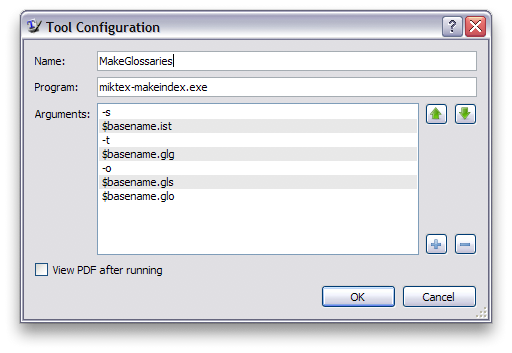
\includegraphics[width=.9\textwidth]{texworks-win_glossaries}

Now \textbf{repeat the above step} for another similar tool called ``\textsf{MakeAcronyms}'', but replace \texttt{thesis.glg} with \texttt{thesis.alg}; \texttt{thesis.gls} with \texttt{thesis.acr}; \texttt{thesis.glo} with \texttt{thesis.acn}.

On Linux and Mac systems, these are equivalent to the command lines

\begin{lstlisting}
makeindex -s <base>.ist -t <base>.glg -o <base>.gls <base>.glo
\end{lstlisting}


\textbf{If you have Perl installed} (likely if you're using Linux or Mac), you can just run

\begin{lstlisting}
makeglossaries <base>
\end{lstlisting}

\noindent and it'll process both the acronyms and the glossaries.

\subsubsection{Tool Configuration for Generating the List of Publications}
Now add a new processing tool called ``\textsf{Create Own Publication List}'' (or some other name). Configure it as shown below:

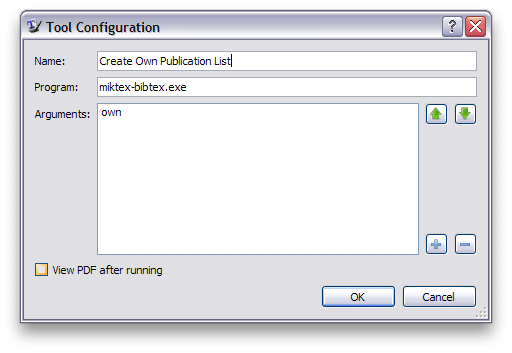
\includegraphics[width=.9\textwidth]{texworks-win_ownpub}


On Linux and Mac systems, these are equivalent to the command lines

\begin{lstlisting}
bibtex own
\end{lstlisting}

If you are using the \texttt{splitpubs} environment for separating your published journal articles and conference proceedings, then you would need to set up similar processors for \texttt{ownjour} and \texttt{ownconf} instead:

\begin{lstlisting}
bibtex ownjour
bibtex ownconf
\end{lstlisting}


\section{Compiling \texttt{thesis.tex}}

The following processing tools/commands are triggered automatically on Overleaf as you edit your file, but you must execute them manually if compiling on your own machine. (The \verb|$| is the terminal command prompt; don't type that!)

\begin{lstlisting}
$  pdflatex thesis
$  bibtex thesis
$  makeglossaries thesis   <-- if you have acronyms and glossaries
$  makeindex thesis  <-- if you have indices
$  pdflatex thesis
$  pdflatex thesis
\end{lstlisting}

You will need to run \texttt{makeglossaries} again if you add and use a \emph{new glossary or acronym entry}.

If you do not have Perl installed on your system (Mac and GNU/Linux systems are likely to already have Perl installed), then you should execute the following commands to replace \texttt{makeglossaries}:

\begin{lstlisting}
$ makeindex -s thesis.ist -t thesis.glg -o thesis.gls thesis.glo
$ makeindex -s thesis.ist -t thesis.alg -o thesis.acr thesis.acn
\end{lstlisting}

\section{Printing from Acrobat Reader}
Remember to set the \textbf{paper size} to \textbf{A4} and \textbf{page scaling} to \textbf{None} in the \textsf{Print} dialog, otherwise the margins would be incorrect.


\section{Using the umalayathesis Class}\label{sec:howto}

\subsection{Activation}\label{sec:activation}
To `activate' the class, make sure your main document file (e.g.\ \texttt{thesis.tex}) starts off with \verb|\documentclass{umalayathesis}|:

\begin{lstlisting}
\documentclass{umalayathesis}
\usepackage{graphicx}
\usepackage{... other packages you need}
\end{lstlisting}


This will set up the page margins, paragraph spacing, indents, page numbers, font face and size, citation and bibliography format, amongst other things.

\subsection{Document Class Options}

Some faculties or departments may have varying, and sometimes conflicting, requirements on various formatting details, which may not have been explicitly described in the official thesis style guidelines. The following document class options may be used to address some of the more commonly requested changes: please also read the commented code in the sample \texttt{thesis.tex} carefully for examples and tips.

\begin{description}
\item[\texttt{english}] (default) English thesis.

\item[\texttt{bahasam}] Malay thesis. At present \texttt{apacite} and \texttt{newapa} has not yet been localised to Bahasa Malaysia.


\item[\texttt{apacite}] (default) Loads the \texttt{apacite} package, which implements the APA
   citation and referencing styles strictly, including expansion of
   of 3--5 authors on first citation.

\item[\texttt{newapa}] Loads the \texttt{natbib} and \texttt{apalike} package for a APA-like reference list
   but \emph{does not fully implement} all APA citation styles. In particular,
   this option will not expand references with 3--5 authors on first citation.
   \textbf{Not recommended unless explicitly requested by examiner}.

\item[\texttt{custombib}] Does not pre-load any bibliography style or packages; you will need to
   specify \verb|\bibliographystyle|, \verb|\bibliographystyleown| etc yourself, or load \texttt{natbib} yourself if necessary. See \ref{sec:custombib} for an example.

\item[\texttt{appendixhead}] Add `APPENDICES' before the first Appendix.

\item[\texttt{altcaption}] Caption in smaller fonts; only Figure X, Table Y bold.

\item[\texttt{singlespacedlisttitles}] Long titles in the ToC, LoT, LoF, LoA are single-spaced.

\item[\texttt{listpageheader}] If your faculty requires a ``header row'' at the top of
   the List of Figures/Tables. You can re-define \verb|\lofpageheader| and
   \verb|\lotpageheader| if necessary, e.g.
          \verb|\renewcommand{\lofpageheader}{\hfill Page}|

\item[\texttt{boldfrontmattertoc}] If your faculty wants front matter ``chapters'' to be
   bold in the ToC.

\item[\texttt{boldbackmattertoc}] If the backmatter ``chapters'' are to be bolded as well.

\item[\texttt{uppercasetoc}] If all ``chapters'' level headings must be upper-cased in the ToC.

\end{description}

If further minor modifications are required, it is recommended to do so with re-issuing commands to change settings or \verb|\renewcommand|, \verb|\patchcmd| etc in the \emph{preamble of \texttt{thesis.tex}}. Modifying \texttt{umalayathesis.cls} directly is discouraged, as far as possible, since this may complicate debugging and future maintenance.


\subsection{Author Information}\label{sec:author:info}
You need to provide some author information in the preamble. Example lines from \texttt{thesis.tex}:

\lstset{language=[LaTeX]{TeX}}
\begin{lstlisting}[moretexcs={submissionyear,submissionmonth,faculty,othertitle,degree,qualification}]
\author{Lim Lian Tze}
\title{My Ground-breaking Research}
\othertitle{Hasil Penyelidikan yang Menggegarkan}
\faculty{Faculty of Amazing Research}
\submissionyear{2012}
\degree{Doctor of Philosophy}
\end{lstlisting}

These information are needed to generate the preliminary pages.

If \verb|\othertitle| is given, then the second abstract will display it
(i.e. if your thesis is `\texttt{english}' then this is printed on top of the Malay abstract.
and if your thesis is `\texttt{bahasam}' then this is printed on top of the English abstract).
If no \verb|\othertitle| is given, then the second abstract will not have any translated thesis title.

If you need to specify your department as well, you may write

\begin{lstlisting}
\faculty{Department of Hyperboles\\Faculty of Amazing Research}
\end{lstlisting}


\subsection{Preliminary Pages}\label{sec:prelim:pages}
Once in the main document body, \verb|\frontmatter| sets up the, well, front matter. This include setting the page numbers to lower-case Roman numerals.

\textsf{umalayathesis} can generate the cover page, title page and original literary work declaration page with the following lines (included in \texttt{thesis.tex}):


\begin{lstlisting}[moretexcs={makecoverandtitlepage,copyrightpage,declarationpage}]
% \makecoverandtitlepage{\mastercoursework}
% \makecoverandtitlepage{\mastermixedmode}
% \makecoverandtitlepage{\masterresearch}
\makecoverandtitlepage{\doctoralresearch}
% \makecoverandtitlepage{\doctoralmixedmode}
\declarationpage
\end{lstlisting}

Please \emph{uncomment} the correct \verb|\makecoverandtitle| line to generate the correct statement on the title page.

\subsection{Acknowledgements}\label{sec:acknowledge}
\lstset{moretexcs={acknowledgements}}
This is provided using \verb|\acknowledgements|:


\begin{lstlisting}
\acknowledgements{I would like to thank my parents, my family, my supervisor...}
\end{lstlisting}

\subsection{Abstract}\label{sec:abstract}
Write your abstracts in separate files (\texttt{sample-abstract.tex} for the English abstract and \texttt{sample-msabstract.tex} for the Malay abstract in this example), and include them in \texttt{thesis.tex} like this:

\begin{lstlisting}[moretexcs={abstractfromfile,msabstractfromfile}]
\abstractfromfile{sample-abstract}
\msabstractfromfile{sample-msabstract}
\end{lstlisting}

\subsection{Table of contents, List of figures and tables}\label{sec:toc}

These are auto-generated by the following lines (included in \texttt{thesis.tex}):

\begin{lstlisting}[moretexcs={tableofcontents,listoftables,listoffigures}]
{\clearpage
\tableofcontents\clearpage
\listoffigures\clearpage
\listoftables\clearpage}
\end{lstlisting}


\subsection{Main Chapters}\label{sec:chapters}

I highly recommend that each chapter be written in a separate file. For example, \texttt{chap-intro.tex} has the contents

\begin{lstlisting}[moretexcs={chapter}]
\chapter{Introduction}
This is the introduction chapter.

\section{Problem Background}
We study the...
\end{lstlisting}


And \texttt{chap-litreview.tex}:

\begin{lstlisting}[moretexcs={chapter}]
\chapter{Literature Review}
We review the state of the art in...

\section{Early Approach}
Researchers first attempted to...
\end{lstlisting}


In \texttt{thesis.tex}, these chapter files are included with the following lines:

\begin{lstlisting}[keepspaces=true,moretexcs=mainmatter]
\mainmatter             % signal start of main chapters
\input{chap-intro}      % no .tex extension!
\input{chap-litreview}
\input{...}
\end{lstlisting}

\subsection{Appendices}\label{sec:appendices}
Again, I recommend keeping each appendix chapter in its own file e.g.~\texttt{app-umldiagram.tex}:

\begin{lstlisting}
\chapter{UML Diagrams}
...
\end{lstlisting}

And in \texttt{thesis.tex}:

\begin{lstlisting}
\begin{appendices}
\input{app-umldiagram}
\input{...}
\end{appendices}
\end{lstlisting}


\subsection{Citations and Bibliography}\label{sec:bibliography}
\textsf{umalayathesis} uses the \textsf{apacite} package with the \texttt{natbibapa} option to format citations and bibliography in the APA style.
Here are some useful variants of the \verb|\cite| command; see the \textsf{apacite} manual for full list.


\bigskip

{\lstset{moretexcs={citeA,citeNP,citeauthor,citeyear}}
\begin{tabular}{>{\textbullet\hspace{6pt}}l @{\hspace{6pt}$\rightarrow$\hspace{6pt}} l}
\verb|\citep{Lim:2009}| & (Lim, 2009)\\
\verb|\citet{Lim:2009}| & Lim (2009)\\
\verb|\citealp{Lim:2009}| & Lim, 2009 (no parenthesis)\\
\verb|\citep[see][p.~7]{Lim:2009}| & (see Lim, 2009, p.~7)\\
\verb|\citeauthor{Lim:2009}| & Lim\\
\verb|\citeyearpar{Lim:2009}| & (2009)\\
\end{tabular}
}

\bigskip

In \texttt{thesis.tex}, these lines will print the bibliography list:

\begin{lstlisting}[keepspaces=true,moretexcs=backmatter]
\backmatter            % signal start of back matter
\bibliography{bibfile} % bibliography file name without .bib extension
\end{lstlisting}


\subsection{List of Publications}

First, make sure that you enter details about your own publications in your \verb|.bib| file.  Then in \verb|thesis.tex|, search for the following line:

\lstset{escapechar={}}
\begin{lstlisting}
\nociteown{Lim:2009}
\end{lstlisting}

Replace the BibTeX key between the curly braces with that of your own publication.  If you have more than one publications, simply separate them with commas inside the curly braces, like this:

\begin{lstlisting}
\nociteown{lim:tang:2004,Lim:2009}
\end{lstlisting}

If you need your publications to be categorised by types (journal articles and conference proceedings), use the \texttt{splitpubs} environment with \verb=\...jour= and \verb=...conf= instead:

\begin{lstlisting}[keepspaces=true,moretexcs={\nociteownjour,\nociteownconf,\bibliographyownjour,\bibliographyownconf},emph={splitpubs},emphstyle={\bfseries}]
\begin{splitpubs}
\nociteownjour{lim:tang:2004}  % journal articles
\nociteownconf{Lim:2009}       % conference proceedings
\bibliographyownjour{myrefs}
\bibliographyownconf{myrefs}
\end{splitpubs}
\end{lstlisting}


\subsection{Glossary}\label{sec:glossary}
You can maintain a consistent glossary and acronym list using the \textsf{glossaries} package. It also supports acronym expansion on first mention!

First, define your acronyms and terms in a separate file e.g.~\texttt{myacronyms.tex}:


\begin{lstlisting}[moretexcs={newacronym,newglossaryentry},
emph={name,description,plural,firstplural},emphstyle=\bfseries]
% \newglossaryentry{label}{name={term},description={explanation}}
\newglossaryentry{lexicon}{
name={lexicon},
description={The vocabulary of a language, including its words and expressions. More formally, it is a language's inventory of lexemes}
}

% \newacronym[description={explanation}]{label}{abbrv}{full form}
\newacronym
[description={single word or words that are grouped in a language's lexicon}]
{LI}{LI}{lexical item}

\newacronym[description={The application of computational linguistics principles to problems}]
{NLP}{NLP}{Natural Language Processing}

% when the plural form is irregular, specify firstplural and plural
\newacronym
[firstplural={parts of speech}, plural={POS},
description={linguistic category of lexical items}]
{POS}{POS}{part of speech}
\end{lstlisting}


Loading the glossary and acronym list, and later printing the list of acronyms and glossary in \texttt{thesis.tex}:


\begin{lstlisting}[moretexcs={loadglsentries,printglossaries,listofacronyms}]
% Must be loaded BEFORE \begin{document}!
\loadglsentries{myacronyms}
\begin{document}
...
% List of acronyms is between list of tables and list of appendices
\listofacronyms\clearpage
...
\bibliography{bibfile}
% Glossaries is placed AFTER the bibliography
% (only entries that are actually used in the text will be listed)
\printglossary
...
\end{lstlisting}


To mention them in the text (i.e.~\texttt{chap-xxx.tex} etc):


\lstset{moretexcs={gls,glsplural,ac,acp,Gls,Glsplural,Ac,Acp}}
\begin{lstlisting}[frame=single]
Let's talk about \acp{LI} and \acp{POS} in \ac{NLP}. I mention again \acp{LI}. We will also talk about \glsplural{lexicon}.
\end{lstlisting}


Notice how the acronyms are expanded on first use, as well as the use of \verb|\glsplural| and \verb|\acp| for plurals:


{\fboxsep=12pt\SingleSpacing
\noindent\fbox{\begin{minipage}{.95\textwidth}
Let's talk about lexical items (LIs) and parts of speech (POS) in Natural
Language Processing (NLP). I mention again LIs. We will also talk about lexicons.
\end{minipage}}
}

You will need to run \texttt{pdflatex}, \texttt{makeglossaries}, then 2 more runs of \texttt{pdflatex} for the glossaries to appear properly.

Use \verb|\Gls|, \verb|\Glsplural|, \verb|\Ac|, \verb|\Acp| etc.~if you need to capitalise the first letter of your terms at the beginning of sentences.

%!TEX ROOT = thesis.tex
\chapter{Introduction}
\section{First Level Heading}

You can use the usual \LaTeX{} commands and environments: footnotes\footnote{See here, how weird, how to fill out an entire line. See here, how weird, how to fill out an entire line. See here, how weird, how to fill out an entire line. See here, how weird, how to fill out an entire line. See here, how weird, how to fill out an entire line. } too\footnote{don't you agree?}, certainly with figures and tables as well.

\begin{figure}[hbt!]\centering
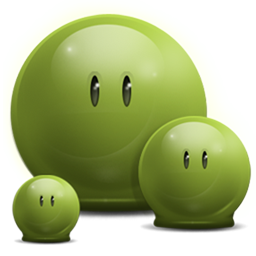
\includegraphics[width=.3\textwidth]{green}
\caption{First figure. OK?}
\end{figure}

\begin{table}[hbt!]
\caption{This is a table.}
\centering
\begin{tabular}{ l c r }
\hline
Hey & How's it & Going?\\ \hline
Fine! & Just great. & See ya!\\
Fine! & Just great. & See ya!\\
\hline
\end{tabular}
\end{table}

This is a quotation:

\begin{quote}
Nam dui ligula, fringilla a, euismod sodales, sollicitudin vel, wisi. Morbi auctor lorem non justo. Nam lacus libero, pretium at, lobortis vitae, ultricies et, tellus. Donec aliquet, tortor sed accumsan bibendum, erat ligula aliquet magna, vitae ornare odio metus a mi. Morbi ac orci et nisl hendrerit mollis. Suspendisse ut massa. Cras nec ante. Pellentesque a nulla.
\end{quote}

You can create subfigures (and similarly subtables.)

\begin{figure}[hbt!]
\begin{minipage}{0.48\textwidth}
  \centering
  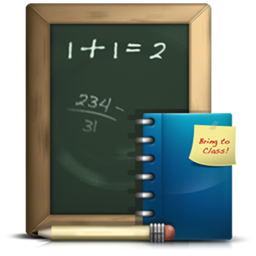
\includegraphics[width=4cm]{school}
  \subcaption{This is a subfigure}
\end{minipage}
%
\hfill
%
\begin{minipage}{0.48\textwidth}
  \centering
  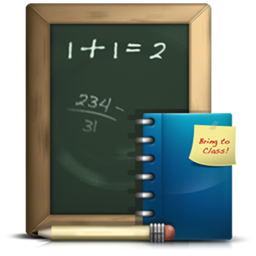
\includegraphics[width=4cm]{school}
  \subcaption{This is another subfigure}
\end{minipage}

\caption[Second figure (caption without citation)]{Second figure.  If you have a citation in the caption, you might want to provide an optional caption that doesn't contain the citation so that it won't appear in the List of Tables or Captions. \cite{audibert:2004}}
\end{figure}



\begin{table}[hbt!]
\caption{A trivial subtable example}

\begin{minipage}{.49\textwidth}
\centering
\subcaption{One Subtable}

\begin{tabular}{l l}
  \hline
  One & Two \\
  \hline
  Three & Four\\
  Five & Six\\
  \hline
\end{tabular}
\end{minipage}
%
\hfill
%
\begin{minipage}{0.49\textwidth}
\centering
\subcaption{Two Subtables}

\begin{tabular}{l l}
  \hline
  $\alpha$ & $\beta$ \\
  \hline
  $\gamma$ & $\delta$\\
  $\epsilon$ & $\zeta$\\
  \hline
\end{tabular}
\end{minipage}

\end{table}

\subsection{Suggestions about Tables}

\LaTeX{} tables can be notoriously\ldots \emph{interesting} to do. But whatever you do, \textbf{please don't nest tabulars} i.e.~put tabulars within tabulars. They are hard to read and debug, and prone to errors.

\url{http://www.tablesgenerator.com} is a handy tool, where you can design your tables and then export the \LaTeX{} code. You can even paste in some data you copied from Excel via the `File > Paste table data' function.

For tables/columns that are too wide to fit nicely on the page, see this blog post for some suggestions:
\url{http://tex.my/how-to-deal-with-wide-tables/}

For tables that are too long and must be broken up into multiple pages, use the \texttt{longtable} or \texttt{supertabular} packages: these have mechanisms for automatically breaking the tables, and repeating the table header/footer rows on each page. Click \href{https://www.overleaf.com/latex/examples/a-longtable-example/xxwzfxkxxjmc}{here} for a \texttt{longtable} example, which is reproduced in Table~\ref{tab:longtable:example}. Table~\ref{tab:supertabular:example} shows a \texttt{supertabular} example.

\subsection{Suggestion about Itemize and Enumerate Lists}

\texttt{umalayathesis} v1.3 loads the \texttt{enumitem} package, which provides some mechanisms for customising lists.

If the space above the \texttt{itemize} and \texttt{enumerate} lists are too big for your liking:
%
\begin{itemize}
  \item This is the first point and
  \item This is the second point
\end{itemize}

You can use the \texttt{nosep} option:

\begin{itemize}[nosep]
  \item This is the first point and
  \item This is the second point
\end{itemize}

To use a different bullet:

\begin{itemize}[label=$\star$]
  \item This is the first point and
  \item This is the second point
\end{itemize}

And even different numbering scheme (you may need to change the list's left margin):

\begin{enumerate}[label=(\roman*),leftmargin=3em]
  \item This is the first point and
  \item This is the second point
\end{enumerate}

Other possible commands for changing the counter format are:

\begin{itemize}
\item \verb|\arabic|: 1, 2, 3, \ldots
\item \verb|\roman|: i, ii, iii, \ldots
\item \verb|\Roman|: I, II, III, \ldots
\item \verb|\alph|: a, b, c, \ldots
\item \verb|\Alph|: A, B, C, \ldots
\end{itemize}

\section{Citations}

\texttt{umalayathesis} uses the \texttt{apacite} package (with \texttt{natbibapa} option) and bibliography style. Use \verb|\citep| for parenthetical citations, such as this one \citep{audibert:2004}. To get text citations, use the \verb|\citet| command and you'll get \citet{audibert:2004}.

Starting with umalayathesis v1.5.1, the APA7 guidelines is out, where first citations with many authors now \emph{do not need to be expanded}. Therefore citations with $3 \leq \text{authors} \leq 5$ are always abbreviated now; e.g. \cite{azarova:etal:2002}.

\subsection{Using Another Bibliography Style}
\label{sec:custombib}

If your faculty allows/requires you to use an entirely different bibliography style, use the \texttt{custombib} document class option. You are then responsible for loading any packages (e.g.~\texttt{natbib}) and setting up the necessary \verb|\bibliographystyle|, etc.

For example, if your faculty requires you to use the \texttt{IEEEtran} bibliography style, you can write

\begin{lstlisting}[language={[LaTeX]TeX},
emph={\bibliographystyleown,\bibliographystyleownjour,\bibliographystyleownconf},
emphstyle=\bfseries]
\documentclass[custombib]{umalayathesis}
\bibliographystyle{IEEEtran}
\bibliographystyleown{IEEEtran}  %% Style for List of Publications
\bibliographystyleownjour{IEEEtran}
\bibliographystyleownconf{IEEEtran}
\end{lstlisting}



\subsubsection{Symbols and Abbreviations}

If you're just starting to write your thesis, you may want to maintain a list of symbols and acronyms, and process it using the \texttt{makeglossaries} command, so that acronyms are automatically expanded/abbreviated, and listed in the List of Symbols and Abbreviations. See the \texttt{umalayathesis-manual.pdf} for further information.
Great. Let's talk about \glspl{LI} and \glspl{POS} in \gls{NLP}. I mention again \glspl{LI}. Oh I have a symbol too, it's \gls{theta}. And I talk a lot about \glspl{lexicon}.

Or if you've actually already nearly finished writing your thesis, it's probably much easier to forget about \texttt{glossaries} and the \texttt{myacronyms.tex} file, and just create a List of Symbols and Abbreviations manually yourself with a tabular:

\begin{lstlisting}[language={[LaTeX]TeX},emph={\chapter},emphstyle=\bfseries]
\chapter{List of Symbols and Abbreviations}
\begin{tabular}{l @{ : } l}
UM & University Malaya\\
KL & Kuala Lumpur\\
\end{tabular}
\end{lstlisting}

\paragraph{A Fifth Level Heading}
This will not be included in the Table of Contents.

Here's an example \texttt{longtable}. Beware: very large long tables can take a loooooong time to compile!

\begin{longtable}[c]{|l|l|l|}
\caption{A sample \texttt{longtable}.} \label{tab:longtable:example} \\

%%% These are the header row on the FIRST page
\hline \multicolumn{1}{|c|}{\textbf{First column}} & \multicolumn{1}{c|}{\textbf{Second column}} & \multicolumn{1}{c|}{\textbf{Third column}} \\ \hline
\endfirsthead

% These are the header row for SUBSEQUENT pages
\multicolumn{3}{c}%
{{\bfseries \tablename\ \thetable{}, continued}} \\
\hline \multicolumn{1}{|c|}{\textbf{First column}} & \multicolumn{1}{c|}{\textbf{Second column}} & \multicolumn{1}{c|}{\textbf{Third column}} \\ \hline
\endhead

% These are the footer row for EACH page EXCEPT LAST
\hline \multicolumn{3}{r}{{Continued on next page}} \\
\endfoot

% These are the footer for the FINAL page
\hline
\endlastfoot

One & abcdef ghjijklmn & 123.456778 \\
One & abcdef ghjijklmn & 123.456778 \\
One & abcdef ghjijklmn & 123.456778 \\
One & abcdef ghjijklmn & 123.456778 \\
One & abcdef ghjijklmn & 123.456778 \\
One & abcdef ghjijklmn & 123.456778 \\
One & abcdef ghjijklmn & 123.456778 \\
One & abcdef ghjijklmn & 123.456778 \\
One & abcdef ghjijklmn & 123.456778 \\
One & abcdef ghjijklmn & 123.456778 \\
One & abcdef ghjijklmn & 123.456778 \\
One & abcdef ghjijklmn & 123.456778 \\
One & abcdef ghjijklmn & 123.456778 \\
One & abcdef ghjijklmn & 123.456778 \\
One & abcdef ghjijklmn & 123.456778 \\
One & abcdef ghjijklmn & 123.456778 \\
One & abcdef ghjijklmn & 123.456778 \\
One & abcdef ghjijklmn & 123.456778 \\
One & abcdef ghjijklmn & 123.456778 \\
One & abcdef ghjijklmn & 123.456778 \\
One & abcdef ghjijklmn & 123.456778 \\
One & abcdef ghjijklmn & 123.456778 \\
One & abcdef ghjijklmn & 123.456778 \\
One & abcdef ghjijklmn & 123.456778 \\
One & abcdef ghjijklmn & 123.456778 \\
One & abcdef ghjijklmn & 123.456778 \\
One & abcdef ghjijklmn & 123.456778 \\
One & abcdef ghjijklmn & 123.456778 \\
One & abcdef ghjijklmn & 123.456778 \\
One & abcdef ghjijklmn & 123.456778 \\
One & abcdef ghjijklmn & 123.456778 \\
One & abcdef ghjijklmn & 123.456778 \\
One & abcdef ghjijklmn & 123.456778 \\
One & abcdef ghjijklmn & 123.456778 \\
One & abcdef ghjijklmn & 123.456778 \\
One & abcdef ghjijklmn & 123.456778 \\
One & abcdef ghjijklmn & 123.456778 \\
One & abcdef ghjijklmn & 123.456778 \\
One & abcdef ghjijklmn & 123.456778 \\
One & abcdef ghjijklmn & 123.456778 \\
One & abcdef ghjijklmn & 123.456778 \\
One & abcdef ghjijklmn & 123.456778 \\
One & abcdef ghjijklmn & 123.456778 \\
One & abcdef ghjijklmn & 123.456778 \\
One & abcdef ghjijklmn & 123.456778 \\
One & abcdef ghjijklmn & 123.456778 \\
One & abcdef ghjijklmn & 123.456778 \\
One & abcdef ghjijklmn & 123.456778 \\
One & abcdef ghjijklmn & 123.456778 \\
One & abcdef ghjijklmn & 123.456778 \\
One & abcdef ghjijklmn & 123.456778 \\
One & abcdef ghjijklmn & 123.456778 \\
One & abcdef ghjijklmn & 123.456778 \\
One & abcdef ghjijklmn & 123.456778 \\
One & abcdef ghjijklmn & 123.456778 \\
One & abcdef ghjijklmn & 123.456778 \\
One & abcdef ghjijklmn & 123.456778 \\
One & abcdef ghjijklmn & 123.456778 \\
One & abcdef ghjijklmn & 123.456778 \\
One & abcdef ghjijklmn & 123.456778 \\
One & abcdef ghjijklmn & 123.456778 \\
One & abcdef ghjijklmn & 123.456778 \\
One & abcdef ghjijklmn & 123.456778 \\
One & abcdef ghjijklmn & 123.456778 \\
One & abcdef ghjijklmn & 123.456778 \\
One & abcdef ghjijklmn & 123.456778 \\
One & abcdef ghjijklmn & 123.456778 \\
One & abcdef ghjijklmn & 123.456778 \\
One & abcdef ghjijklmn & 123.456778 \\
One & abcdef ghjijklmn & 123.456778 \\
One & abcdef ghjijklmn & 123.456778 \\
One & abcdef ghjijklmn & 123.456778 \\
One & abcdef ghjijklmn & 123.456778 \\
One & abcdef ghjijklmn & 123.456778 \\
One & abcdef ghjijklmn & 123.456778 \\
One & abcdef ghjijklmn & 123.456778 \\
One & abcdef ghjijklmn & 123.456778 \\
One & abcdef ghjijklmn & 123.456778 \\
One & abcdef ghjijklmn & 123.456778 \\
One & abcdef ghjijklmn & 123.456778 \\
\end{longtable}

\clearpage
Here's a \texttt{supertabular} example too.

\begin{center}
\topcaption{A sample \texttt{supertabular}.} \label{tab:supertabular:example}

%%% These are the header row on the FIRST page
\tablefirsthead{%
  \hline \multicolumn{1}{|c|}{\textbf{First column}} & \multicolumn{1}{c|}{\textbf{Second column}} & \multicolumn{1}{c|}{\textbf{Third column}} \\ \hline
}

% These are the header row for SUBSEQUENT pages
\tablehead{%
  \multicolumn{3}{c}%
  {{\bfseries \tablename\ \thetable{}, continued}} \\
  \hline \multicolumn{1}{|c|}{\textbf{First column}} & \multicolumn{1}{c|}{\textbf{Second column}} & \multicolumn{1}{c|}{\textbf{Third column}} \\ \hline
}

% These are the footer row for EACH page EXCEPT LAST
\tabletail{%
  \hline \multicolumn{3}{r}{{Continued on next page}} \\
}

% These are the footer for the FINAL page
\tablelasttail{\hline}

\begin{supertabular}[c]{|l|l|l|}
One & abcdef ghjijklmn & 123.456778 \\
One & abcdef ghjijklmn & 123.456778 \\
One & abcdef ghjijklmn & 123.456778 \\
One & abcdef ghjijklmn & 123.456778 \\
One & abcdef ghjijklmn & 123.456778 \\
One & abcdef ghjijklmn & 123.456778 \\
One & abcdef ghjijklmn & 123.456778 \\
One & abcdef ghjijklmn & 123.456778 \\
One & abcdef ghjijklmn & 123.456778 \\
One & abcdef ghjijklmn & 123.456778 \\
One & abcdef ghjijklmn & 123.456778 \\
One & abcdef ghjijklmn & 123.456778 \\
One & abcdef ghjijklmn & 123.456778 \\
One & abcdef ghjijklmn & 123.456778 \\
One & abcdef ghjijklmn & 123.456778 \\
One & abcdef ghjijklmn & 123.456778 \\
One & abcdef ghjijklmn & 123.456778 \\
One & abcdef ghjijklmn & 123.456778 \\
One & abcdef ghjijklmn & 123.456778 \\
One & abcdef ghjijklmn & 123.456778 \\
One & abcdef ghjijklmn & 123.456778 \\
One & abcdef ghjijklmn & 123.456778 \\
One & abcdef ghjijklmn & 123.456778 \\
One & abcdef ghjijklmn & 123.456778 \\
One & abcdef ghjijklmn & 123.456778 \\
One & abcdef ghjijklmn & 123.456778 \\
One & abcdef ghjijklmn & 123.456778 \\
One & abcdef ghjijklmn & 123.456778 \\
One & abcdef ghjijklmn & 123.456778 \\
One & abcdef ghjijklmn & 123.456778 \\
One & abcdef ghjijklmn & 123.456778 \\
One & abcdef ghjijklmn & 123.456778 \\
One & abcdef ghjijklmn & 123.456778 \\
One & abcdef ghjijklmn & 123.456778 \\
One & abcdef ghjijklmn & 123.456778 \\
One & abcdef ghjijklmn & 123.456778 \\
One & abcdef ghjijklmn & 123.456778 \\
One & abcdef ghjijklmn & 123.456778 \\
One & abcdef ghjijklmn & 123.456778 \\
One & abcdef ghjijklmn & 123.456778 \\
One & abcdef ghjijklmn & 123.456778 \\
One & abcdef ghjijklmn & 123.456778 \\
One & abcdef ghjijklmn & 123.456778 \\
One & abcdef ghjijklmn & 123.456778 \\
One & abcdef ghjijklmn & 123.456778 \\
One & abcdef ghjijklmn & 123.456778 \\
One & abcdef ghjijklmn & 123.456778 \\
One & abcdef ghjijklmn & 123.456778 \\
One & abcdef ghjijklmn & 123.456778 \\
One & abcdef ghjijklmn & 123.456778 \\
One & abcdef ghjijklmn & 123.456778 \\
One & abcdef ghjijklmn & 123.456778 \\
One & abcdef ghjijklmn & 123.456778 \\
One & abcdef ghjijklmn & 123.456778 \\
One & abcdef ghjijklmn & 123.456778 \\
One & abcdef ghjijklmn & 123.456778 \\
One & abcdef ghjijklmn & 123.456778 \\
One & abcdef ghjijklmn & 123.456778 \\
One & abcdef ghjijklmn & 123.456778 \\
One & abcdef ghjijklmn & 123.456778 \\
One & abcdef ghjijklmn & 123.456778 \\
One & abcdef ghjijklmn & 123.456778 \\
One & abcdef ghjijklmn & 123.456778 \\
One & abcdef ghjijklmn & 123.456778 \\
One & abcdef ghjijklmn & 123.456778 \\
One & abcdef ghjijklmn & 123.456778 \\
One & abcdef ghjijklmn & 123.456778 \\
One & abcdef ghjijklmn & 123.456778 \\
One & abcdef ghjijklmn & 123.456778 \\
One & abcdef ghjijklmn & 123.456778 \\
One & abcdef ghjijklmn & 123.456778 \\
One & abcdef ghjijklmn & 123.456778 \\
One & abcdef ghjijklmn & 123.456778 \\
One & abcdef ghjijklmn & 123.456778 \\
One & abcdef ghjijklmn & 123.456778 \\
One & abcdef ghjijklmn & 123.456778 \\
One & abcdef ghjijklmn & 123.456778 \\
One & abcdef ghjijklmn & 123.456778 \\
One & abcdef ghjijklmn & 123.456778 \\
One & abcdef ghjijklmn & 123.456778 \\
\end{supertabular}
\end{center}

% \texttt{umalayathesis} is English by default. If you need to writeyour thesis in Malay, start with \verb|\documentclass[bahasam]{umalayathesis}| instead. This is currently experimental: You may need to customise some other things on your own; e.g.~checking through if \texttt{apacite} is fully localised to Malay. If you'd like to contribute your translations, take a look at section 6.2 of the \href{http://texdoc.net/pkg/apacite}{apacite documentation}.

%!TEX ROOT = thesis.tex
\chapter{Dummy Chapter}

Hello!!\index{furball}

\begin{figure}[hbt!]
\centering Test 3
\caption{Let's see. What have we got here?}
\end{figure}


\bibliography{myrefs}

%% Use these lines, if you need a single list of own publications
% Make sure you have defined your own papers in the .bib file!
\nociteown{Lim:2009,Bond:etal:WordNetBahasa:2014}
\bibliographyown{myrefs}

%% Use these lines, if your list of own publications needs to be split
%% into "Journal articles" and "Conference proceedings"
% Make sure you have defined your own papers in the .bib file!
% \begin{splitpubs}
%   \nociteownjour{Bond:etal:WordNetBahasa:2014}
%   \nociteownconf{Lim:2009}
%   \bibliographyownjour{myrefs}
%   \bibliographyownconf{myrefs}
% \end{splitpubs}

\begin{appendices}
%!TEX ROOT = thesis.tex
\chapter{Manuals, Technical Specifications, Documentations, Example Scenarios}

%!TEX ROOT = sample.tex
\chapter{Try}

\lipsum[1-2]

\end{appendices}

%% Comment out this line if you do not have a separate glossary.
% \printglossary

\end{document}
